\documentclass{article}\usepackage[]{graphicx}\usepackage[]{xcolor}
% maxwidth is the original width if it is less than linewidth
% otherwise use linewidth (to make sure the graphics do not exceed the margin)
\makeatletter
\def\maxwidth{ %
  \ifdim\Gin@nat@width>\linewidth
    \linewidth
  \else
    \Gin@nat@width
  \fi
}
\makeatother

\definecolor{fgcolor}{rgb}{0.345, 0.345, 0.345}
\newcommand{\hlnum}[1]{\textcolor[rgb]{0.686,0.059,0.569}{#1}}%
\newcommand{\hlsng}[1]{\textcolor[rgb]{0.192,0.494,0.8}{#1}}%
\newcommand{\hlcom}[1]{\textcolor[rgb]{0.678,0.584,0.686}{\textit{#1}}}%
\newcommand{\hlopt}[1]{\textcolor[rgb]{0,0,0}{#1}}%
\newcommand{\hldef}[1]{\textcolor[rgb]{0.345,0.345,0.345}{#1}}%
\newcommand{\hlkwa}[1]{\textcolor[rgb]{0.161,0.373,0.58}{\textbf{#1}}}%
\newcommand{\hlkwb}[1]{\textcolor[rgb]{0.69,0.353,0.396}{#1}}%
\newcommand{\hlkwc}[1]{\textcolor[rgb]{0.333,0.667,0.333}{#1}}%
\newcommand{\hlkwd}[1]{\textcolor[rgb]{0.737,0.353,0.396}{\textbf{#1}}}%
\let\hlipl\hlkwb

\usepackage{framed}
\makeatletter
\newenvironment{kframe}{%
 \def\at@end@of@kframe{}%
 \ifinner\ifhmode%
  \def\at@end@of@kframe{\end{minipage}}%
  \begin{minipage}{\columnwidth}%
 \fi\fi%
 \def\FrameCommand##1{\hskip\@totalleftmargin \hskip-\fboxsep
 \colorbox{shadecolor}{##1}\hskip-\fboxsep
     % There is no \\@totalrightmargin, so:
     \hskip-\linewidth \hskip-\@totalleftmargin \hskip\columnwidth}%
 \MakeFramed {\advance\hsize-\width
   \@totalleftmargin\z@ \linewidth\hsize
   \@setminipage}}%
 {\par\unskip\endMakeFramed%
 \at@end@of@kframe}
\makeatother

\definecolor{shadecolor}{rgb}{.97, .97, .97}
\definecolor{messagecolor}{rgb}{0, 0, 0}
\definecolor{warningcolor}{rgb}{1, 0, 1}
\definecolor{errorcolor}{rgb}{1, 0, 0}
\newenvironment{knitrout}{}{} % an empty environment to be redefined in TeX

\usepackage{alltt}
\usepackage[margin=1.0in]{geometry} % To set margins
\usepackage{amsmath}  % This allows me to use the align functionality.
                      % If you find yourself trying to replicate
                      % something you found online, ensure you're
                      % loading the necessary packages!
\usepackage{amsfonts} % Math font
\usepackage{fancyvrb}
\usepackage{hyperref} % For including hyperlinks
\usepackage[shortlabels]{enumitem}% For enumerated lists with labels specified
                                  % We had to run tlmgr_install("enumitem") in R
\usepackage{float}    % For telling R where to put a table/figure
\usepackage{natbib}        %For the bibliography
\bibliographystyle{apalike}%For the bibliography
\IfFileExists{upquote.sty}{\usepackage{upquote}}{}
\begin{document}

In lecture 16, we looked at precipitation amounts in Madison County (at 
Morrisville station). We found that the Weibull distribution had a good fit
to the monthly precipitation amounts.\\

We found that the MLEs for the Weibull distribution were 
\begin{align*}
    \hat{a}&=2.1871\\
    \hat{\sigma}&=3.9683
\end{align*}
and
\[-\mathcal{L}(\{\hat{a}, \hat{\sigma}\}|\mathbf{x}) = 2166.496\]
is the realized negative log-likelihood.
Note this means that the log-likelihood is
\[\mathcal{L}(\{\hat{a}, \hat{\sigma}\}|\mathbf{x}) = -2166.496,\]
and the usual likelihood is
\[L(\{\hat{a}, \hat{\sigma}\}|\mathbf{x}) = e^{\left[\mathcal{L}(\{\hat{a}, \hat{\sigma}\}|\mathbf{x})\right]} \approx = e^{-2166.496},\]
which \texttt{R} cannot differentiate from 0.

\begin{enumerate}
  \item Someone asked ``why Weibull?" in class. That is, why wouldn't we use 
  another right-skewed distribution like the Gamma (see Lecture 15), or
  the Log-Normal (see Lecture 17).
  \begin{enumerate}
    \item Compute the MLEs for these data using a Gamma distribution.
    
    \textbf{Solution:} The MLEs for the Gamma distribution are: 
    \[\hat{\alpha} = 4.1761\]
    \[\hat{\beta} = 0.8406\]
    
    \item Compute the MLEs for these data using the Log-Normal distribution.
    
    \textbf{Solution:} The MLEs for the Log-Normal distribution are: 
    \[\hat{\alpha} = 1.1313\]
    \[\hat{\beta} = 0.5333\]
    
    \item Compute the likelihood ratio to compare the Weibull and the Gamma distribution. 
    Which has a better fit according to the likelhiood ratio?
    \[Q = \frac{L(\{\hat{a}, \hat{\sigma}\}|\mathbf{x})}{L(\{\hat{\alpha}, \hat{\beta}\}|\mathbf{x})}=e^{\left[\mathcal{L}(\{\hat{a}, \hat{\sigma}\}|\mathbf{x}) - \mathcal{L}(\{\hat{\alpha}, \hat{\beta}\}|\mathbf{x})\right]}\]
    
    \textbf{Solution:} The likelihood ratio for the Weibull and the Gamma distribution is $Q = \ensuremath{2.161379\times 10^{-7}}$. As $Q < 1$, we can conclude that the denominator is greater than the numerator. As the denominator is greater, we can conclude that the Gamma distribution is a better fit of a distribution for this data.
    
    
    \item Compute the likelihood ratio to compare the Weibull and the Log-Normal distribution.
    Which has a better fit according to the likelihood ratio?
    \[Q = \frac{L(\{\hat{a}, \hat{\sigma}\}|\mathbf{x})}{L(\{\hat{\mu}, \hat{\sigma}\}|\mathbf{x})}=e^{\left[\mathcal{L}(\{\hat{a}, \hat{\sigma}\}|\mathbf{x}) - \mathcal{L}(\{\hat{\mu}, \hat{\sigma}\}|\mathbf{x})\right]}\]
    
    \textbf{Solution:} The likelihood ratio for the Weibull and the Log-Normal distribution is $Q = \ensuremath{2.370633\times 10^{16}}$. As $Q > 1$, we can conclude that the numerator is greater than the denominator. As the numerator is greater, we can conclude that the Weibull distribution is a better fit of a distribution for this data.
    
    
    \item Compute the likelihood ratio to compare the Gamma and the Log-Normal distribution.
    Which has a better fit according to the likelhiood ratio?
    \[Q = \frac{L(\{\hat{\alpha}, \hat{\beta}\}|\mathbf{x})}{L(\{\hat{\mu}, \hat{\sigma}\}|\mathbf{x})}=e^{\left[\mathcal{L}(\{\hat{\alpha}, \hat{\beta}\}|\mathbf{x}) - \mathcal{L}(\{\hat{\mu}, \hat{\sigma}\}|\mathbf{x})\right]}\]
    
    \textbf{Solution:} The likelihood ratio for the Gamma and the Log-Normal distribution is $Q = \ensuremath{1.096815\times 10^{23}}$. As $Q > 1$, we can conclude that the numerator is greater than the denominator. As the numerator is greater, we can conclude that the Gamma distribution is a better fit of a distribution for this data.
    
  \end{enumerate}
  
\textbf{Summary:} The Gamma distribution is best distribution, Weibull is the second best distribution, and Log-Normal distribution is third best.
  
  \begin{figure}[H]
  \begin{center}
  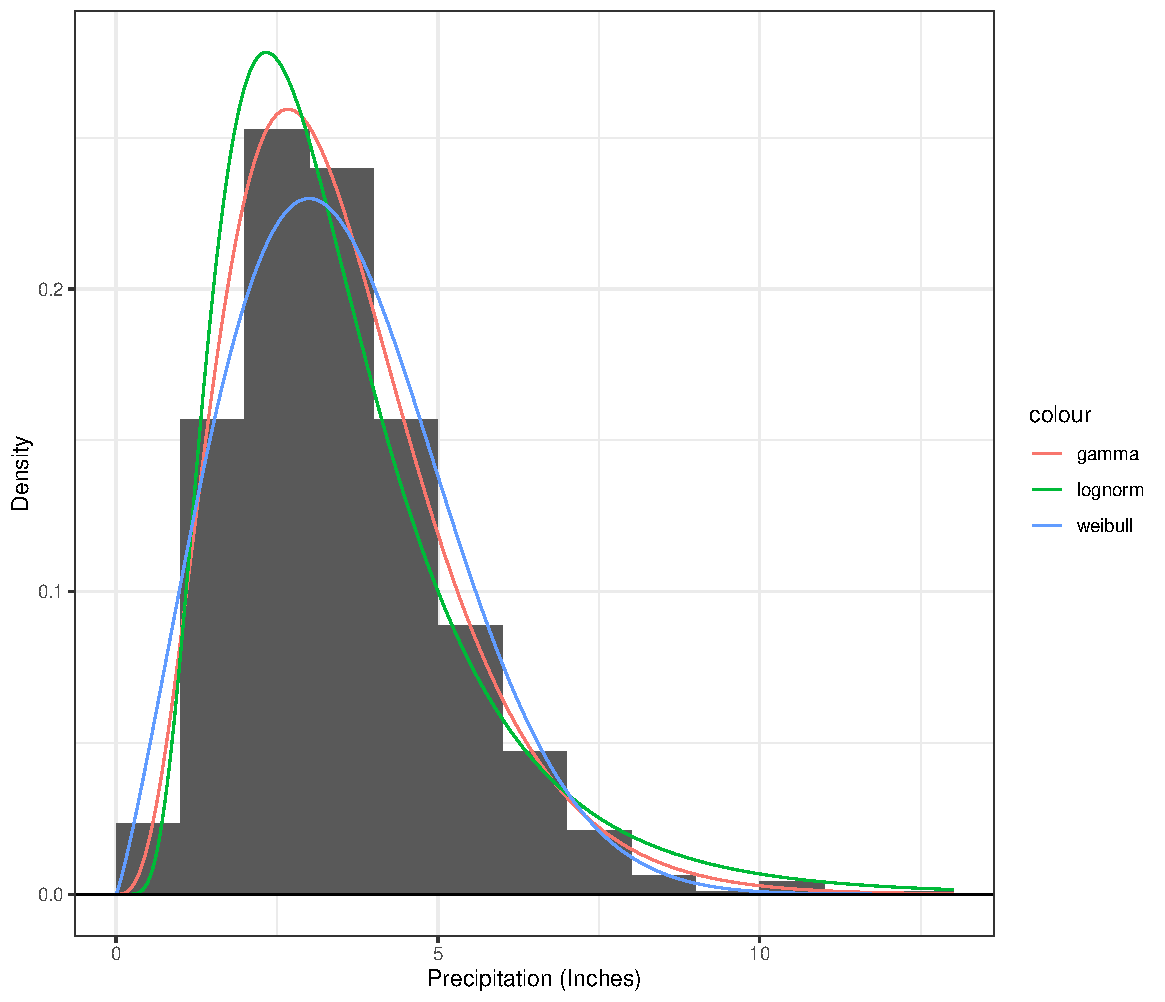
\includegraphics[width=\textwidth]{Rplot.pdf}
  \caption{Distribution Of Precipitation}
  \label{Rplot}
  \end{center}
\end{figure}
  
  
  \item Optional Coding Challenge. Choose the ``best" distribution and refit the
  model by season.
  \begin{enumerate}
    \item Fit the Distribution for Winter (December-February).
    \item Fit the Distribution for Spring (March-May).
    \item Fit the Distribution for Summer (June-August).
    \item Fit the Distribution for Fall (September-November).
    \item Plot the four distributions in one plot using \texttt{cyan3} for Winter,
    \texttt{chartreuse3} for Spring, \texttt{red3} for Summer, and \texttt{chocolate3}
    for Fall. Note any similarities/differences you observe across the seasons.
  \end{enumerate}
\end{enumerate}

\bibliography{bibliography}
\end{document}
